\documentclass[a4paper, 11pt]{article}

\usepackage[margin=1.5in]{geometry}

\usepackage[english]{babel}
\usepackage[utf8]{inputenc}
\usepackage{amsmath}
\usepackage{graphicx}
\usepackage{subcaption}
\usepackage{gensymb}
\usepackage{float}
\usepackage{scrextend}
\usepackage{lastpage}
\usepackage{fancyhdr}
\usepackage{cite}
\usepackage{url}
\usepackage[colorinlistoftodos]{todonotes}

%\pagestyle{myheadings}
\pagestyle{fancy}
\setlength{\headheight}{13.6pt}

\lhead{Team \# 56361}                                      %%%%%%%%%%%%%%%%%%%%INSERT TEAM NUMBER HERE
\rhead{Page \thepage \ of \ \pageref{LastPage}}
\lfoot{}
\rfoot{}
\cfoot{}

\newcommand{\block}[1][3]{\begin{addmargin}{#1em}}
\newcommand{\pictureblock}[1][-8]{\begin{addmargin}{#1em}}
\newcommand{\blockend}{\end{addmargin}}
\newcommand{\img}[1][0]{\includegraphics[scale = 0.35]{#1}}
\fancypagestyle{firststyle}{
  \lhead{Team \# 56361}                                       %%%%%%%%%%%%%%%%%INSERT TEAM NUMBER HERE
  \rhead{Page \thepage \ of \ \pageref{LastPage}}
  \lfoot{}
  \rfoot{}
  \cfoot{}
}


\title{Insert Title}
\author{Insert Team Number}
\date{\today}
\begin{document}

\tableofcontents
\newpage
\thispagestyle{firststyle}


% The judges will evaluate the quality of your writing in the Solution Paper:

% · Conciseness and organization are extremely important.

% · Key statements should present major ideas and results.
%       WE NEED TO ENSURE WE HAVE THIS CHUNK

%   
%
% · Present a clarification or restatement of the problem, as appropriate.
%        WE NEED THIS ONE.
%

% · Present a clear exposition of all variables, assumptions, and hypotheses.
%        This is in progress   

% · Present an analysis of the problem, including the motivation or justification for the model that is used.
%       I think this one is mostly done. 

% · Include a design of the model.
%       This is on going, but going well. 

% · Discuss how the model could be tested, including error analysis and stability (conditioning, sensitivity,etc.).
%        This is needed desperately. 

% · Discuss any apparent strengths or weaknesses in your model or approach.
%         This is planned. 


\section{Introduction}
\subsection{Problem}

Every day millions of people drive on toll roads. Every second they spend wasting their time stuck in toll plazas merging is multiplied by how many drivers are on the road. This means that every day countless years of peoples lives are lost stuck in toll plazas. This means that improving toll plaza efficiency even a little bit saves a lot, and every improvement counts. An easy way to improve toll plaza speed and safety is by making the toll plazas very wide. This is a problem though, because wide toll plazas would be dramatically expensive. Thus we need to optimize safety and throughput while making it as cost effective as possible. 

To perform this optimization, we have created a comprehensive artificial intelligence network to simulate cars driving through a toll plaza, including individual lane changing and optimizing for safety. This is considered a multi-agent system, where each agent is optimizing for itself, while still producing results that can be applied globally. In the traffic engineering terminology, it is a micro-simulation, as we are modeling traffic on the car level, rather than on a higher level. This means our results are applicable to a variety of scales. 

When designing toll plazas, we considered two main factors. The first factor that we considered was shape. This is the overall structure of the toll plaza, and how they come together. The second factor was `merging patterns'. These were custom designed systems of double white lines and related structures to influence the drivers to merge in a particular way at a particular time. 

These two systems, our artificial intelligence, and our various toll plaza designs, allowed us to explore many different possibilities, and allowed us to find a toll plaza design that surpassed the most common design in every way measured. 

% What are barrier tolls

% B booth lanes merge into L highway lanes
% Bottleneck problem
% Optimize a recovery area (in shape, size, and merging pattern) to minimize this problem
% Define merging pattern
%%In choosing this method, we created a microsimulation to represent traffic moving through the "fan in" region of a toll plaza. A microsimulation is defined by the Department of Transportation as "the modeling of individual vehicle movements on a second or subsecond basis for the purpose of assessing the traffic performance of highway and street systems" \cite{guidelines}. 



\subsection{Assumptions}
% \textbf{Do we allow the cars entering the simulation to form queues?} %why a question?
% We assume that a car will choose the toll lane with the shortest queue when approaching a toll island, regardless of the lateral location of each lane. This assumption allows us to ignore the shape, size, and merging pattern of the toll plaza approach zone, focusing instead on the effectiveness of the departure zone design. Dubedi et al. (2012) show that drivers choose toll lanes based on queue lengths, number of heavy vehicles in each queue, and  number of lanes a driver would have to cross to get to a given queue \cite{LaneChoice}. They also claim that the most important factor, by far, is queue length. 

In our approach of the problem, we had 8 main assumptions.

The first assumption was that the cars are uniform in size and only occupy one node at a time. This means that a car is never straddling two lanes as it merges or changes lanes. This limits our ability to see realistic collisions within our simulation, but we will discuss an alternative method to assess collision risk in Section \ref{model_design} of our paper.

The second assumption is that cars will only change lanes if there is an explicit reason to do so, based on lanes merging and nearby cars. We assume that there is nothing gained by changing lanes without one of these factors prompting a car to do so, since each car's objective is to reach the end of the toll plaza. 

The third assumption is that there are no laws dictating what type of vehicles or what speed vehicles may travel in specific lanes. This is unlike highways with passing lanes or HOV lanes. We justify the lack of a left passing lane because we are studying the recovery zone of toll plazas, where all vehicles are picking up speed and attempting to merge into any open lane. A passing lane would be impractical for this purpose. 

The fourth assumption is that a car will enter any given tollbooth with equal probability. The findings of Dubedi et al. (2012) in \textit{Modeling Automobile Drivers' Toll-Lane Choice Behavior at a Toll Plaza} support this assumption as long as the toll plaza is not located near a highway entrance or exit \cite{LaneChoice}. Technically this assumption carries another: that we are sufficiently far away from either an entrance or exit. 

The fifth assumption is that all lanes are parallel. They do not curve into each other to merge, but they simply travel in the same direction until one lane ends. Although lanes do not merge like this in the real world, this suffices for our model because when one lane merges into an adjacent lane smoothly, only one car can occupy the merge zone at a given time. 

The sixth assumption is that electronic toll collection booths, such as those using transponders, do not require drivers to stop or slow down. We also assume that the capacity of an electronic toll collection system is limited only by the speed of the cars moving through. Only one car can exit the booth at a time, but once it has exited, another car is free to exit immediately. 

The seventh assumption is that the area of land that a toll plaza recovery zone occupies determines the cost of construction. We do not calculate explicit price estimates, but we do attempt to limit the size of our recovery zones in order to minimize costs. 

The eighth assumption is that 10\% of the cars are autonomous. We are not optimizing our design for the present, but taking into account current technology trends. It is predicted that by 2032, half of new cars produced will be autonomous \cite{autonomous_cars}. Accounting for the gradual transition that this will lead to, we believe 10 \% is a good standard to consider in our design. 

\section{Model Design}
\label{model_design}

\subsection{Process}

The design process progressed in several stages. We first considered the desired features which we required. These features included the ability to measure throughput and analyze traffic, as well as danger. We also wanted the ability to model different kinds of cars driving through the system, both self-driven and human-driven. We ultimately decided on an almost entirely deterministic simulation. The artificial intelligence that we ultimately settled on was entirely deterministic. The only amount of non-determinism in our solution was the cars emerging from the tollbooths. Since it was uniform, and our simulations occurred over a long time scale, the simulations eventually reach an equilibrium. This means that in many scenarios, for certain variables, we did not need to compute means, because from run to run, they would be identical. 

These requirements led to the development of the main idea behind our model, a multi-agent system model where each agent maximizes its utility as determined primarily by three factors. 
The first factor is safety, each agent wants to remain safe. What defines safe evolved as we added complexity to the model. This is discussed in depth in Section \ref{ai_design}. 
The second factor is an agent's distance to the lane end. If a lane is ending soon, the agent desires to leave that lane and is incentivized to do so. This is further discussed in the Subsection \ref{ai_impl}.  
The third factor is speed, each agent desires to go as fast as possible, up to the speed limit (plus a factor which determines if they drive faster than the speed limit). Further discussion can be found in the Subsection \ref{ai_impl}. 

For our agents, we used the standard Observe, Act, Update model. This is where each actor \textit{observes} the world, chooses an \textit{action}, and then the world state is simultaneously \textit{updated}.  

For the world in which the agents lived, we initially considered two distinct worlds. 

The first world was a graph based structure denoting links between the places in which the agents could live. This has several nice properties, for example, we could model lanes merging as places where two `columns' of nodes both have the same single column of nodes as a parent. 
But this world has two main downsides. The first downside is searching the area. Each agent needs to be able to understand the area around it, which we found to be computationally complex. The second downside is the fact that visualizing this area is difficult, as is generating the various worlds. 

The second world was a 2D array based structure where some locations are marked as out of bounds. This had several upsides, primarily that it was computationally efficient to search the layout, and that visualizing the system was easier. The downside is that more exotic merging patterns were not possible. 

Ultimately the upsides of the 2D array based method won out, with the main choice being influenced by the computational efficiency, as well as the visualization. The visualization was distinctly important, as it allowed us to understand and debug the model as needed. Additionally, the use of a 2D array allowed us to define the distance between lattices as approximately 15 feet, and each timestep to have a length of 1 second. This means that high way speeds of 60 miles per hour corresponds to 6 units forward per second. Therefore our model allows for the cars to reach highway speeds. 


\subsubsection{The AI Design Process}
\label{ai_design}
Our development of the artificial intelligence system used to simulate car behavior proceeded in a few stages. In the first stage,
a simple utility function was defined for each car, which only took into account information regarding that car and 
the local road structure near it. The second stage involved a more complex utility function for each car which took into account the cars around it, 
with the intended goal of reducing collisions. The third stage introduced a light predictive element, in that the cars attempted to 
predict where nearby cars were headed. 

This subsection shall present the motivations for these distinct stages, and why each is not a final solution to the problem, 
while the corresponding subsection in Section~\ref{model_design} will present the details for the functionality of the final solution.  

As previously stated, the first stage began with only a simple utility function. 
In order to define what each car should do, it is sufficient to define what they want. This process is most effectively 
captured by the notion of a utility function, where a number is assigned to each world state and to each possible action.
We have a notion of an \textit{action}, which is a single choice that the driver can make. 
The choice is simply whether the car will change lanes or accelerate.
This information, along with the car's location, is sufficient for determining the utility function, 
at least in this early stage. 

This method works surprisingly well in simple scenarios. When no lane changes are needed, each car moves forward with no alterations to its current route, 
as we have biased the cars towards staying in their own lanes. This was useful for prototyping. It served as a good initial step, as it allowed us to validate our time step system, as well as ensure 
we have a minimal working model. 

However, shortcomings arise immediately when lane changes are needed, occurring when a lane ends. This immediately results in collisions. 
The failings meant that this model was unacceptable. 

The second utility function took into account the relative positions of the other cars, without taking into account where the cars were moving. 
The most important effect of this change was the prevention of a car colliding into one in front of it, or switching lanes 
and running into another car. The significant aspect of this is that the cars took note of \textit{relative} positions, which enabled them to react 
to the area around them. It did not allow them to react to the actions of cars. 

The primary downfall of this model was that cars would move into the same location. This is an inevitable issue with this utility function, but it can 
be easily avoided by the next modification, which is light predictive power.

The third stage added predictive power to each of the cars. We designed this so the `prediction' was simply each car noting where the 
other cars could likely go, and tending to avoid those places. By avoiding the places other cars could be soon, collisions are avoided. 
This model of predicting where the cars could go closely replicates the human model of prediction, as humans tend to avoid others in traffic by not driving 
into where someone else will be soon. 

Additionally, we had a variety of parameters that allowed us to affect how the cars behaved. A few of these parameters were 
designed to simulate self-driving cars. This will be discussed in Section \ref{ai_impl}.

This was our final stage in the AI design process, as the cars avoided accidents and successfully merged into lanes as appropriate. More details for 
each stage will be discussed in Section \ref{model_design}, as they relate to implementation. 

\subsection{The Model}

Our model can be broken up into two distinct pieces. The first of these pieces is the simulation. The second piece is the evaluation and analysis of the simulation. These pieces are decoupled, which means that the analysis is entirely separate from the simulation, ensuring that our analysis is not designed to fit the simulation. Our discussion of the model shall be broken into chunks corresponding to these pieces. 

The low-level details of the simulation shall be discussed in sections \ref{lane_top} (Merging Pattern) and \ref{ai_impl} (Artificial Intelligence). % list others as they come up.

The evaluation and analysis of the model will be discussed in sections \ref{collision_risk} (Assessing Accident Prevention), \ref{cost_delay} (Assessing Throughput, Delay, Cost). % list others as they come up.

\subsubsection{Merging Patterns}
\label{lane_top}

In real life road systems, there are a variety of systems in place to ensure that drivers do not move from one lane to another. These include double-white lines, as well as double-white lines with diagonal white lines (hence forth called double-white-diagonals) in them. Each indicator has varying levels of severity, with double-white diagonals being `bad' to cross, while double-white-diagonals would be `catastrophic'. 

These systems are an important factor in determining the effectiveness of a particular merge pattern following a toll plaza. Double-white lines are how a traffic engineer guides the flow of traffic. We have reflected this in our model, by the system that we have named the \textit{Merging Pattern system}. 
In our model, each location on the road is represented as a RoadNode object.
A RoadNode represents a place that a car could live. Each RoadNode has a `left preference' (preference to change to the left lane) and a `right preference' (preference to change to the right lane), which describes a utility modifier for the agents. These left and right preferences are encoded as integer values. These preferences manifest themselves in the model in the utility functions of the driver, by biasing the driver towards a particular action, i.e. drivers do not want to cross the double white line because they can see it. We found this to be a simple and effective way of creating merging patterns. 


\subsubsection{Artificial Intelligence}
\label{ai_impl}

As discussed in Section \ref{ai_design}, at the core of the artificial intelligence is a utility maximization system. This section shall discuss the details of this utility system, as well as the parameters which we use to customize the drivers' behavior. We shall discuss how we use these parameters to distinguish between `self-driving cars', and cars which are driven by `humans', and make an argument that this is a reasonable way to distinguish between them. 

The utility system is based on a series of preferences. The first preference is a preference for not performing illegal actions, where an illegal action is driving off of the road. We have conditions in place which assign extreme negative utility to the practice of driving off the road. 

The second preference is a \textit{lane change} preference. 
Unless the merging pattern (for more information, see Section \ref{lane_top}) determines otherwise, the drivers have a weak preference for not changing lanes. This is based on the idea that changing lanes takes effort, and they would not want to do so unless there is a reason. For choosing to remain in the current lane, the agent gets 9 utility points, while for the left and right lanes, the agent receives 8 utility points. These values are modified by the merging pattern. Additionally for each choice of left and right, a small random factor is added to force the drivers to have a preference for one direction over the other in case all other factors are equal. 

The third preference is speed. Each driver has a preference towards staying near the speed limit, encapsulated in the equation:

\begin{center}
$-|\mbox{DesiredSpeed} - \mbox{AfterActionSpeed}|$
\end{center}

This value is highest when the car's after action speed is closest to their desired speed, meaning the cars attempt to always be near this speed. 

The fourth preference is to not be near the end of a lane. If an agent is 2 seconds away from running out of road, then they have a strong preference to move. If they are 3 seconds away, they still have a strong preference to avoid this area, but it is slightly weaker than if they were 2 seconds away.

These 4 preferences describe the preferences of a driver alone in the world. However, this is far from sufficient to describe how agents should move with respect to each other. These preferences are the \textit{blind} preferences, as they do not see other cars. 

To create the preferences to optimize with respect to the other drivers, let us consider two agents, Agent \textit{A} and Agent \textit{B}, where both agents want to move to location $(x,y)$. Assume that Agent \textit{A} has utility $k_A$ to move there, Agent \textit{B} has $k_B$, and $k_A > k_B$. Agent \textit{A} performs a search and discovers that Agent \textit{B} also wants to move to $(x,y)$ and modifies its utility for that location to $k_A - k_B$. Agent \textit{B} does the same thing, and gets $k_B - k_A$. Since $k_A > k_B$, Agent $B$ will have a higher utility to go elsewhere, and therefore the collision will be avoided. 

This process is repeated for every car within range of another. By predicting where the other cars will go, the cars naturally avoid each other.%%

In order to customize behavior and create a distinction between the self-driving cars and the `manual' cars, we created a variety of parameters for the agents. These parameters are:

\begin{itemize}
\item \textit{recklessness}: Recklessness encapsulates the desire of the driver to cross over restricted merging patterns. As an easy analogy, a reckless driver will drive over double white lines. This is implemented by modifying the effect that the merging pattern has on the driver's utilities. The self-driving cars will have a recklessness of 0, to indicate that they never drive over the double white lines. 
\item \textit{acceleration}: This is how fast the car can accelerate and reflects the differences in the cars. It also serves as a distinction between the self-driving and manual cars. We have decided to assign the self-driving cars a higher acceleration to reflect the simultaneous acceleration of many self-driving cars in a line. 
\item \textit{law abiding speed}: This is the difference between the agent and the speed limit. A car with a higher law abiding speed will want to drive faster, and one with a lower law abiding speed will drive slower. This reflects both preferences for following the law, and the nature of self-driving cars, which will always follow the law. 
\end{itemize}

These variables encode varying preferences, and allow the various cars on the road to be behave differently. 

\subsubsection{Assessing Accident Prevention}
\label{collision_risk}



In optimizing the structure of a toll plaza recovery zone, we aim to minimize the risk of collision. We base our method for assessing collision risk on the one presented by Li et al. (2016) for calculating collision risks at freeway interchange merge areas. Since these structures serve a similar function as tollbooth recovery zones, we assume that the types of collision risks that Li et al. identify can be applied directly to our model. 

We consider two sources of risk: rear-ending and lane changing collisions. These are identified as the most common collisions that can be mitigated by improving the design of merging areas \cite{crashRisk}. Rear-end collisions can occur between two cars in the same lane, when the back car is traveling faster than the car ahead of it. Lane change collisions can occur when a car in a merging lane is traveling alongside a car in the adjacent lane. If the two cars continue to travel side-by-side, a collision can occur when the two lanes merge into one. 

For each type of potential collision, we are concerned with the time until a collision could occur between two cars. For potential rear-end collisions, the time to collision (TTC) can be determined by 

\begin{equation}
\mbox{TTC} = \frac{\mbox{distance between cars}}{\mbox{relative speed}}
\end{equation}

For potential lane change collisions, the TTC can be determined by
\begin{equation}
\mbox{TTC} = \frac{\mbox{distance from lane end}}{\mbox{speed}}
\end{equation}


In our model, a car computes a rear-end TTC calculation at every time step if there is a car less than 100 feet ahead of it that is moving at a slower speed. A car also computes a lane change TTC calculation at every time step if it is less than 150 feet away from the end of its own lane and there is a car beside it in the next lane. This differs slightly from the model created by Li et al. who only consider a TTC calculation between two cars once, when this value is at its minimum. For this reason, we expected that our model would generate many more TTC values than Li's model and thus a significantly higher risk index, as we will discuss further in the Section \ref{results}. 

After each TTC calculation, an assessment of the collision risk is identified using Table \ref{fig:ColRisk} \cite{crashRisk}. 
 
\begin{center}
\begin{table}[h!]
\centering
\begin{tabular}{|c|c|}
\hline
Collision Type & Threshold \\
\hline
Serious Rear End & 0 - 2.8 \\
\hline
General Rear End & 2.8 - 4.7 \\
\hline
Serious Lane Change & 0 - 2.3 \\
\hline
General Lane Change & 2.3 - 4.2 \\
\hline
\end{tabular}

\caption{For each TTC calculation, these threshold values are used to identify a risk level \cite{crashRisk}}
\label{fig:ColRisk}
\end{table}
\end{center}

Each risk identification contributes to an overall count of serious rear-end risks (RES), general rear-end risks (REG), serious lane change risks (LCS), or general lane change risks (LCG). At the end of each traffic simulation we compute the following collision risk index (HCRI) from Li et al. 

\begin{equation}
\mbox{HCRI} = 0.299 \cdot \mbox{LCS} + 0.161 \cdot \mbox{LCG} + 0.3348 \cdot \mbox{RES} + 0.2052 \cdot \mbox{REG}
\end{equation}

Li describes this as the hourly collision risk index. We do not attempt to scale the value we obtain to an hourly index because, as previously stated, our method of determining collision risks produces a significantly higher risk index. However, we use this risk index to compare the relative safety of different merging patterns. 

\subsubsection{Assessing Throughput, Delay, and Cost}
\label{cost_delay}
We aim to maximize throughput, minimize delay, and minimize cost. Delay and throughput are calculated explicitly. We do not optimize for cost directly, but we implicitly consider cost in limiting the length of our recovery zone to 1500 feet, which we chose based on a standard toll plaza model in \textit{Toll Plaza Design} \cite{tollDesignBook}. Once we optimize the design for throughput, delay, and collision risk, we will discuss the potential costs of our design in more detail. 

We calculate throughput for each simulation by counting the number of cars that reach the end of the toll plaza. Inherently, this is straightforward to calculate, but it is an important factor in optimization since it determines the revenue brought in by the toll plaza. 

We define total delay as the difference between the time it takes cars to travel down the length of the recovery zone without having to merge (B = L) and the time it takes for cars to travel the length of the recovery zone with merging (B $>$ L). This describes the delay caused by a given merging pattern, shape, and size. 
In assessing the costs and benefits of each design, we also consider relative delays caused by changes in travel time due to changing the design while holding B and L constant. 




\subsubsection{Heavy and Light Traffic, Varying Toll Collection}

In order to model heavy and light traffic, we first observed that during heavy traffic, the max speed is far lower. To simulate this, we have capped the max speed for heavy traffic scenarios at half the speed for the low traffic scenarios. 

There are two main types of tolls:
automated (EZ-Tag or other such transponder based technology) or manual (exact change or conventional). The difference between exact change and conventional is negligible when compared to the automated systems, and therefore we are only going to consider two types: automated and manual. We identified the chief characteristic between the automated systems and the manual systems: automated systems allow the cars to drive through the toll at full speed, while in manual systems, cars must stop. This manifests itself simply in our model by beginning agents in automated lanes at their maximum speed.
Additionally, manual lanes have a low probability of a car appearing at any given second (between $\frac29$ and $\frac16$). These values come from estimates of the capacity of these types of tollbooths, which for manual tollbooths are between 600 and 800 vehicles per hour \cite{EconomicEvaluation}. As mentioned in the assumptions, we consider the automated tollbooths to have unlimited capacity, so cars can appear from these lanes every time the lane entrance has an opening (or less frequently to simulate lighter traffic). 


\section{Results and Discussion}
\label{results}


We shall begin by discussing preliminary results. This consists primarily of discussing varying shapes and sizes of the model (this will be elaborated on). This gives us a benchmark for when we begin discussing alternate shapes and merging patterns. We shall evaluate each design on safety, speed and throughput throughout, but leave the discussion of costs to the end of the results section.

In this preliminary section discussing bench marks, what will shall consider is \textit{only} different shapes, with varying number of tollbooths, and exiting lanes. First, we shall consider the simplest scenario, which is that the number of tollbooths (B) and the number of exiting lanes (L) are equal. We use L = 5 to examine this case where each tollbooth is an automated booth. While an unrealistic scenario for a toll plaza, we expected this to give us a useful upper bound on the throughput as well as a lower bound for travel time, allowing us to compute delays caused by merging.

\begin{figure}[H]
\begin{center}
\begin{tabular}{c c}
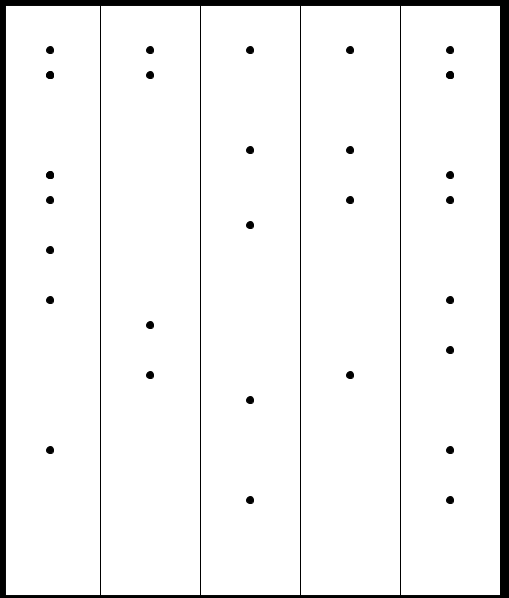
\includegraphics[scale=0.2]{Images/5By5One.png} &
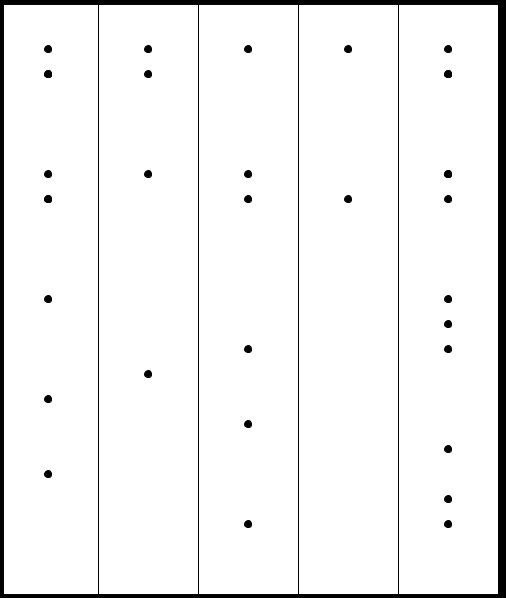
\includegraphics[scale=0.2]{Images/5By5Two.png}
\end{tabular}
\end{center}
\caption{These images represent traffic flow from 5 tollbooths into 5 highway lanes. The image on the right is one time step after the image on the left. The cars begin at the top and move towards the bottom.}
\label{fig:5By5}
\end{figure}
% Need to explain the visualization.

We calculated the throughput for this particular simulation to be 1682, that is, 1682 cars in 360 time steps of our simulation (each of which is 1 second). This corresponds to a throughput of 3364 vehicles per hour per lane. For highway traffic in general, this falls within the regime of forced flow, where cars are forced to slow down due to the varying actions of other cars and create a traffic jam \cite{herman}. The problem of forced flow means that maximizing throughput and minimizing delay times can be competing factors. However, since maximizing throughput is an important goal in designing toll plazas, if we can find merging patterns or different shapes with good throughput relative to this, then we have found a successful toll plaza design, one worth considering as our final recommendation.


% ez tag 5 by 5, 100 long 
%     briefly evaluate the cost vs throughput argument
%     this paragraph has delay time. Make it bench mark


%
%%
%%Andy, mention Figure 1 before you talk about Figure 2
%%
%

Before considering statistics, consider Figure \ref{fig:5By5}. This is a visualization of our model and shows the structure of the world space which the cars live in. As you can see here, the cars in this simulation live somewhere with no lanes ended. In other figures, you will be able to see the shape of where the cars live, as well as approximately the density. 

Consider Figure \ref{fig:ez55}, which shows the histograms of the travel times associated with this particular model. As you can see, this illustrates that the travel times are between 21 and 28 seconds for cars to reach the end of the toll plaza, 
which corresponds to average speeds for each car between 36 mph and 50 mph, which seems reasonable. %%%%
The mean travel time, 23.4 seconds, will be used as a benchmark to compute delays caused by merging B automated booth lanes into L highway lanes. 

We also use this configuration as a benchmark for assessing the safety of other designs for automated tollbooths. 
%%%%%%%
% Andy 
% say that we consider it dimensionless
%%%%%%%
The HCRI value was found to be 57. We adjust this risk index by dividing by the throughput so that we can assess the risk per car moving through our system. For this system we found a 0.0339 risk index per vehicle. 

%% ADD THIS SOMEWHERE ELSE? BUT IT DOESN'T REALLY FIT HERE -K 
%As the toll plaza fills up, the agents need to be more careful, which corresponds to slower speeds. 


\begin{figure}[H]
\begin{center}
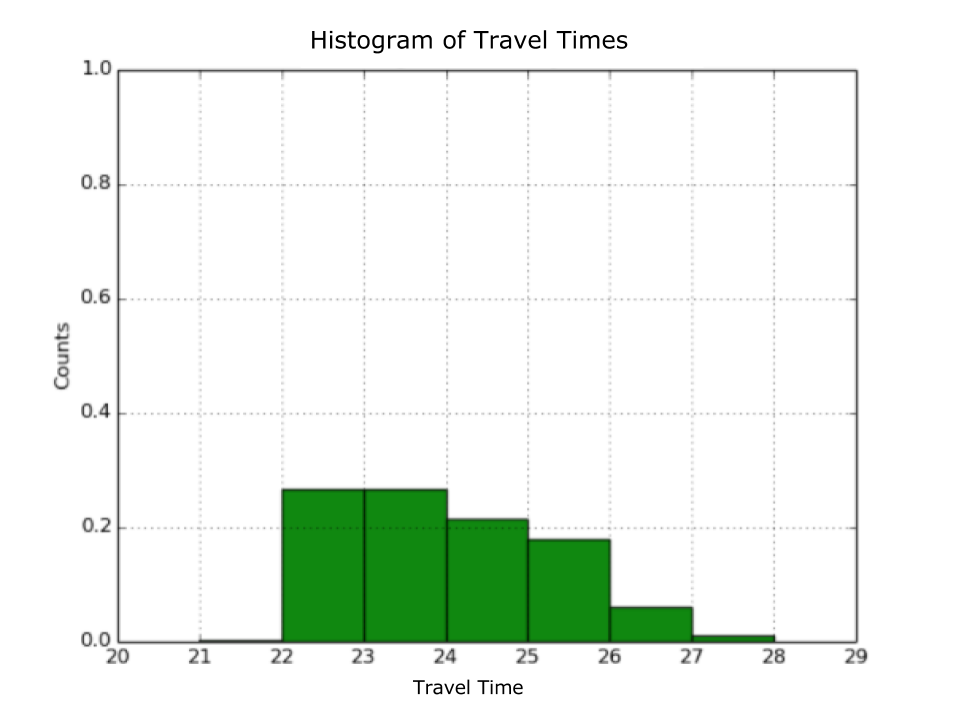
\includegraphics[scale=0.25]{Images/55_ez.png}
\caption{Travel times for L = 5, B = 5 baseline case for automated tollbooths. Mean is 23.4 seconds. }
\label{fig:ez55}
\end{center}
\end{figure}

\begin{figure}[H]
\begin{center}
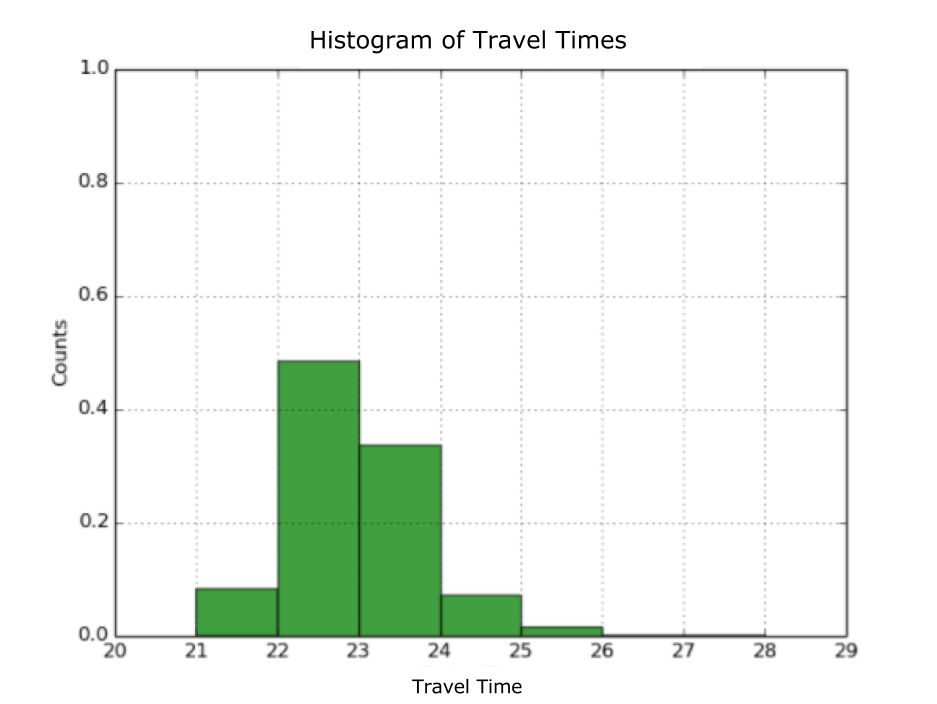
\includegraphics[scale=0.3]{Images/55_man.png}
\caption{Travel times in seconds for the L = 5, B = 5 baseline case for manual tollbooths. Mean is 22.5 seconds.}
\label{fig:manual55}
\end{center}
\end{figure}

% manual 5 by 5, 100 long. HCRI = 52, 0.139 adjusted
% this paragraph has delay time. Make it bench mark
Additionally, we have computed throughput for the manual tollbooths, obtaining a value of only 373 cars. This corresponds to a scaled throughput of 746 vehicles per hour per lane. This is dramatically lower than the automated system. This is to be expected however, as the manual booths let far fewer cars through per time step. As can be seen in Figure \ref{fig:manual55}, it %%%Define "it"
has a similar travel time profile, with the exception that the average speeds tend to be slightly higher. The mean travel time is 22.5 seconds, shorter than the baseline for automated tollbooths presumably because of the lower quantity of cars. Despite this improved average speed, if we were to measure the entire system (i.e. people waiting at the tollbooths), the automated model wins out, due to its extremely high throughput. 

%Probably pretty bad.
The HCRI for this configuration was found to be 52. Adjusted for throughput, we found a risk index of 0.139 per vehicle. This adjusted risk index is higher than that of the automated tollbooth, perhaps because the cars exiting manual tollbooths have to accelerate to highway speed, whereas cars exiting automated tollbooths move more uniformly.
It is important to note that this assessment only shows that there is lower risk associated with automated tollbooths when there is no merging. 

\begin{figure}[H]
\begin{center}
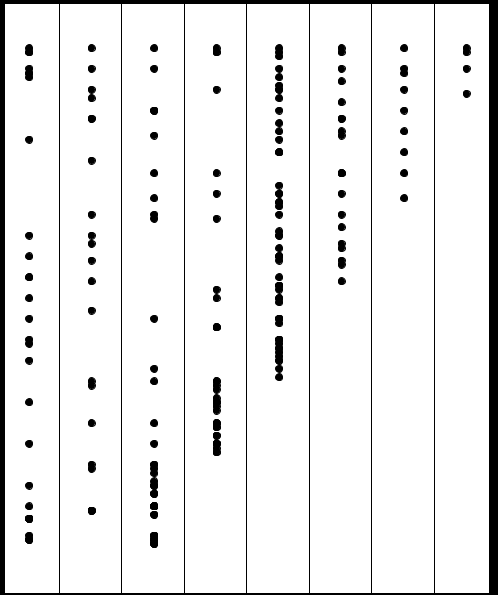
\includegraphics[scale=0.25]{Images/3By8LeftOne.png}
\end{center}
\caption{The image represents traffic flow from 8 tollbooths into 3 highway lanes from top to bottom. }
\label{fig:3By8RightTri}
\end{figure}

\begin{figure}
\begin{center}
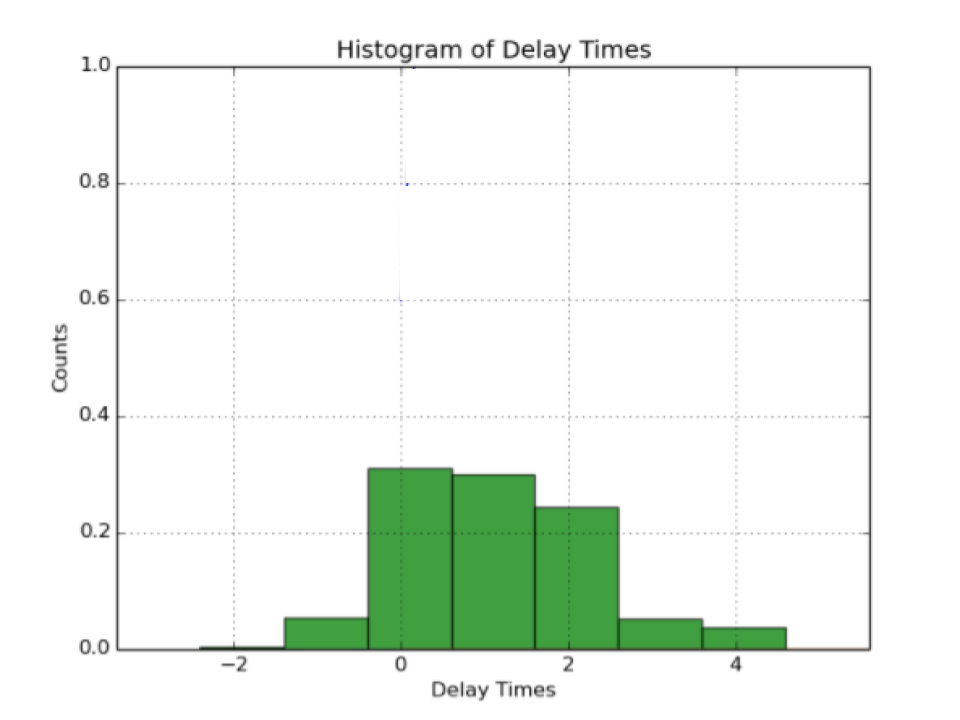
\includegraphics[scale=0.30]{Images/38hist.png}
\caption{A histogram showing the travel times for B = 8, L = 3. The delay times (in seconds) are relative to the benchmark for all manual tollbooths. Mean is 21.0 seconds.}
\label{fig:manual38}
\end{center}
\end{figure}

%Isaac
%  ADDRESS Costs

Now we consider more realistic shapes for the tollbooths, beginning with 8 tollbooths dwindling down to 3 lanes. 
This has the shape of a classical toll plaza, where the cars start spread out, and lanes are removed from the right, resulting in a right triangle shape. 
The general shape (and traffic flow), can be seen in Figure \ref{fig:3By8RightTri}. For manual tollbooths, the travel time for this scenario, where the length of the toll plaza is the same as the 5 by 5, is 21.0 seconds. This means that the right triangle recovery zone did not create any delay, but was 1.5 seconds faster. 
This can be scene in further detail in the histogram (Figure \ref{fig:manual38}). The throughput for this shape is 188 cars, a factor of 2 less than the 5 by 5 manual tollbooth. Adjusting for the number of entrance lanes (B = 8), we find that the throughput is 235 vehicles per tollbooth per hour. We adjust for B rather than L because the result demonstrates the revenue potential for each tollbooth. The adjusted throughput is a factor of 3 lower than the baseline. For this configuration, the HCRI was 129.8. The adjusted risk index was 0.690 per vehicle. It was expected that this risk index would be higher than the baseline (0.139 per vehicle) because collisions are much more likely when cars are forced to merge. 

For the automated tollbooths, we get similarly excellent performance on the travel times, with a mean of 21.4 seconds. This is 2 seconds faster than the baseline. 
The throughput is much higher though, at 1012 cars. Again we adjust for the number of entrance lanes, and we find that the throughput is 1265 vehicles per hour per tollbooth. This is also lower than the baseline throughput (for automated systems) by approximately a factor of 3. The HCRI was 1728.6. Adjusted for throughput, the risk index is 1.71 per vehicle. In this case, it makes sense that the adjusted risk index is higher for the automated tollbooths than the manual tollbooths because the cars merge at higher speeds, which is more dangerous. 








%
% Exotic Shapes
%

\begin{figure}[H]
\begin{center}
\begin{tabular}{c c}
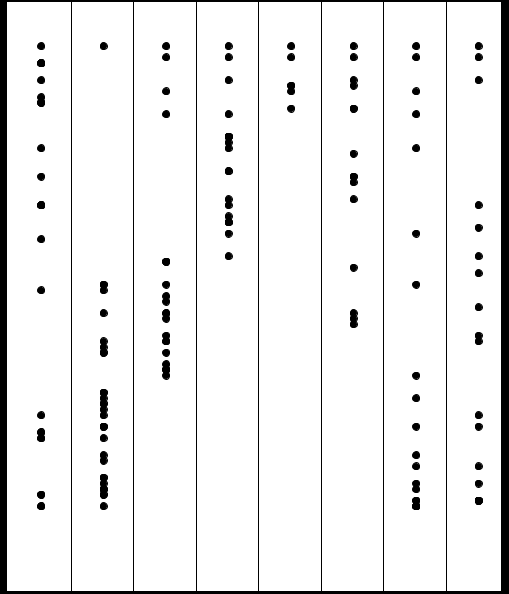
\includegraphics[scale=0.23]{Images/4By8MidTriOne.png} & 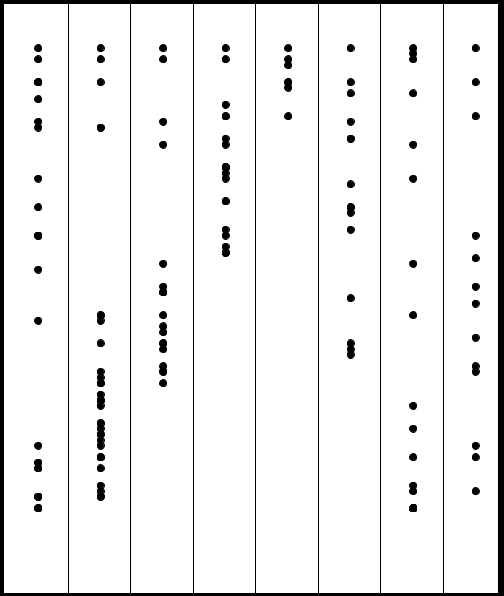
\includegraphics[scale=0.23]{Images/4By8MidTriTwo.png}
\end{tabular}
\end{center}
\caption{The two images represent traffic flow from eight tollbooths into four traffic lanes, where the image on the right is one time step ahead of the image on the right. Where the cars stop appearing is where the traffic lane ends. }
\label{fig:48_split}
\end{figure}

For an original shape, we first present what we have referred to as the 8-4 split system. It's topology can be seen in Figure  \ref{fig:48_split}. After the lanes split apart, the idea is that the lanes quickly comes together. This is not considered in our model, as any such design would have very simple merging procedures. 

% Isaac, include the 48 split. Make a caption about how where the cars aren't is where the lanes end. Do a side by side one. 
%     make sure the label is correct.

%% Isaac can you read these two paragraphs and make sure they don't contradict each other... You might have to change some of the wording because I think they are both true and important... But I don't think both would seem possible to a reviewer. 

This one was examined initially for several reasons. The primary reason was that we wanted drivers to have more options as to where to go at several critical locations during the merging process. We suspected that the right triangle design was quite dangerous and inconvenient for cars in the booth farthest from the continuing lanes. We hypothesized that it would be much safer for cars in the center to change lanes because they would have to make fewer lane changes to arrive in a continuing lane and because they would be able to choose a direction after assessing traffic flow. This, we also thought, might improve travel times and throughput as well. 

Upon careful examination of Figure \ref{fig:48_split}, it is apparent that the center division divides the traffic flow in half. This split means the drivers have less flexibility, which enables them to optimize better. This is a classic scenario in game theory, where each actor optimizing independently results in a worse situation for everyone, and therefore by limiting choices, the \textit{local} optimum more closely aligns with the \textit{global} optimum. This is indeed what we find happens. 

% need to talk about cost
For the manual tollbooths, the throughput was 579 cars, comparable to the adjusted 5 by 5 rectangular plaza with manual tolls. The adjusted throughput for that was 724 vehicles per hour per tollbooth. This is a factor of 3 higher than the 8-3 lane merge using the right triangle design, meaning that the throughput is much better for the 8-4 split system. 
%% ANDY I NEED THE TRAVEL TIME FOR THIS. t = 19.8 s
The mean travel time for cars for this configuration was 19.8 seconds. This is lower than the 8-3 right triangle design by 1.2 seconds, which means that this is another benefit of the 8-4 split design. 
The HRCI for this was only 127.1. Adjusted for throughput, the risk index is 0.220 per vehicle. This is also a factor of 3 better than the risk index for the 8-3 right triangle design (0.690). Each of these criteria is improved by the 8-4 split (compared to the 8-3 right triangle design) when the toll plaza uses manual toll collection. 
% need to comment on how safe this really is, relative to the others. 

% need to talk about relative risk and cost. t = 20.2 s
After computing the throughput for this shape with the automated tollbooths, we found that the throughput was 2716 cars. This is an incredibly high throughput, even for the 8 lane adjusted throughput of 3395 cars per hour per tollbooth. %%%
This means that the throughput for this set up is actually slightly higher than could be seen with an identical optimal model, purely based on the fact that isolating the drivers means they feel more safe, so they can go faster. Additionally, the 8-4 split design is also safer in the case of automated tollbooths. The HCRI is 1362. We adjusted this to a risk index of 0.401 per vehicle. This means that the 8-4 split design is a factor of 4 safer for electronic tollbooths.  The average travel time is also faster, with an average travel time of 20.2 seconds. This is faster than \textit{any} of our shapes, even the purely rectangular shape, for the case of automated toll booths. 

In conclusion of the discussion of this split lane system, it is faster, safer, and cheaper than the alternatives. It is an overall and complete improvement relative to the triangular lane plaza shapes. 

Apart from limiting the length of our merging area, our model hasn't accounted for the costs of implementing any particular design. Since this design optimizes throughput, speed, and safety of a toll plaza, we will now consider the costs further. The area of land that this recovery zone requires is greater than the area needed for the right triangle shape because of the opening it leaves in the center of the highway. Assuming that each lane is 12 feet across and that our design would leave 4 open lanes, there would be a space that is at least 48 feet wide, with a length that can be controlled by adjusting the location at which the outer lanes merge back together. However, we believe that any additional costs due to this opening can be offset by building a gas station or a rest area inside of it. To do this, one would probably have to widen the opening between the outer lanes, which can be flexible, just like the length of the area. This strategy would allow drivers to take a left exit in order to access the facility, and it has been used in Connecticut and Texas, at least. This strategy has the potential to increase the total profit of the toll plaza, even though the plaza structure would cover more land than the right triangle design. Therefore, we do not believe that cost is a prohibiting factor in implementing the lane split approach.  

One thing to note is that all merging patterns that occur are entirely emergent. There are no `double white lines' or other such objects in this shape. Therefore we believe that it is possible to further improve this design through the introduction of double white lines, and we choose to focus on the merging patterns exclusively on this shape. 

\subsubsection{A Shape with Merging Patterns}

The use of double white lines and other lane restrictions causes the traffic flow to progress in a certain way. This is useful for many purposes, as it allows for the traffic flow to be customized. As discussed in the above section, frequently when choices are limited, a greater global optimum can be reached, and the double white lines inherently restrict free choice. As can be seen in Figure \ref{fig:merge_patterns}, we added double white lines to the split toll plaza shape discussed earlier. This had several benefits.

In the Figure \ref{fig:merge_patterns}, you can see that the double white lines do not extend particularly far. However, they serve an important ability, which is that they force the drivers to not crowd the middle, where the important lane changing needs to happen. Even just a small change like this causes the throughput to go up, because when the drivers feel more safe, they can go faster. This is a strong benefit, and can be seen in the various summary statistics that we computed. 



\begin{figure}[H]
\begin{center}
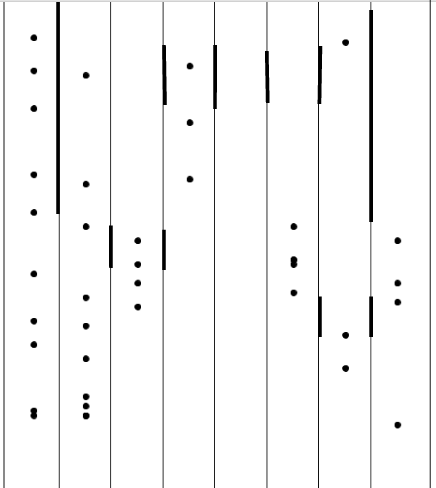
\includegraphics[scale=0.27]{Images/DoubleWhiteLines.png}
\end{center}
\caption{The image represents traffic flow from 8 tollbooths to 4 lanes with double white lines in place. The double white lines are represented by the bold black lines in the image. }
\label{fig:merge_patterns}
\end{figure}
% Isaac, put the graph with the double white lines here. label merge_patterns
% Add something about how the double white lines are thick black instead for visibility
% Make it an H so it is right here.

% need to discuss costs here too
First, we shall consider the manual tollbooth system. For this, we have a throughput of 567 cars, or 709 cars per hour per tollbooth. Although slightly higher, this is comparable to the standard split shape (724 cars per hour per tollbooth). Additionally, we calculated a HCRI score of 127, or 0.179 per vehicle. Again, this is comparable to the standard split shape (0.220) but slightly lower. The merging pattern system though really shines when we consider the travel time, which is 19.5 seconds, the best of all models. This means that this shape and prescribed merging pattern works excellent for optimizing all variables. 

Now we shall consider the automated tollbooth scenario. For this, we once again have excellent throughput, a throughput of 2705 cars, or 3381 cars per hour per tollbooth. This is comparable, although slightly lower, than the throughput of the standard split shape (3395 cars per hour per tollbooth) for the automated scenario. The travel time is also excellent, at only 20.1 seconds, it is among the fastest we have measured, even with the extreme density of the automated tollbooth scenario. The risk index is 0.387 (HCRI = 1310), safer than the scenario with no white lines. This is an excellent result, and optimizes most of the variables. However, where this particular scenario truly shines is that it comes at (basically) no additional expense after the standard split design is built.  

Since this scenario is excellent on on all fronts, we have decided that it is our official recommendation for a toll plaza design. This shall be more formally stated, with discussions of how to generalize this for arbitrary $B$ and $L$ in Section \ref{final_rec}. 




\subsection{Sensitivity Analysis}

In the following section on sensitivity analysis, we cover the proportion of self-driving cars. All other assumptions about constants are supported by citations, and are therefore sensitivity analysis is not needed. 


In our main simulations, the proportion of self-driving cars to regular cars is kept constant at 10\%.
To test how sensitive our results are with this assumption, we are going to run the simulation for the splitting with merging patterns%%%
(the last scenario discussed in the results section) with 9\% of the cars being self driving, as well as 11\%. This should illuminate whether the sensitivity is dramatic. Each of the following is run in the manual traffic scenario, as the smaller number of cars helps exaggerate the effect of the self-driving parameters. During heavy traffic scenarios, the self-driving cars (and all of the cars) are restricted in their actions dramatically, decreasing the difference being self driving and non-self driving. 

For the 9\%, we found that by decreasing the number of self-driving cars on the road, the risk index goes up to 132.14. This is to be expected. The throughput is higher, presumably because the non-self driving cars car sometimes `speed', at 582 cars. 

When considering 11\%, the risk index went down to 123.6, indicating that self-driving cars in our model tend to be safer. This is an excellent validating result, as well as confirming that the HCRI is not particularly sensitive to the number of self-driving cars. The throughput has also decreased, to 548 cars, likely for similar reasons that it increased above. %%
These results indicate that throughput is not sensitive to self-driving car proportions.

Since both relationships are linear, with pretty low changes, we can conclude that the our choice of self-driving car proportion was not particularly significant. Furthermore we validated that the self-driving cars performed as expected.

\section{Conclusion}


\subsection{Model Strengths}
Our microsimulation exhibited key traffic features. Upon inspection, the cars moved at reasonable speeds and changed lane appropriately. No cars became stuck indefinitely. In fact, the travel times for all cars in our simulations were within seconds of each other, exhibiting no clear outliers. Collectively, cars sorted themselves efficiently through merging areas at low traffic levels. In high traffic, the roads surpassed their critical density and traffic jams began to occur. These features correspond to individual and collective behaviors exhibited by cars on highways. This behavior is emergent, it is not programmed into the simulation. This means that the individual intelligence of the drivers closely reflects real life drivers. Every macro-level property of our simulation is emergent from the individual optimization of each driver, just like real life traffic flow. This close reflection of reality, as well as the strong equilibrium which are reached is a great strength of our model. 

Another strength of our simulation is that our final design, the split shape with enforced merging patterns, performed better in throughput, delay, and safety, compared to designs that are standard for toll plazas. We assess that these improvements may come at a greater cost to construct, but our design is flexible enough that we can create usable space between outer lanes for gas stations or rest areas. 

\subsection{Model Weaknesses}
The main weakness of our model is that it is not continuous.  Due to computational costs, we had to limit the number of nodes on our roads. This limited our ability to account for small differences among cars in acceleration, speed, and position. Since our nodes were 15 feet apart, it didn't make sense to account for the sizes of individual cars, which we would have liked to consider in our model. 

%
%
%
%
%
%

%%ANDY AUTONOMOUS CAR

A weakness of our model is the autonomous cars. Although they exhibit the behaviors of autonomous vehicles (rule following, speed matching, others), they do not distinguish themselves a sufficient amount from the `human' driven cars. This is a difficult problem for a micro-simulation or multi-agent system model, as both the human driven cars and the self-driven cars are at their core simulated by code. Therefore making a meaningful distinction is difficult. The behavior of the cars does stand out, but not perhaps to the degree that is desirable. 
%
%
%
%
%
Cost is a potential weakness in our final design. Since the structure takes up a greater area than traditional merge zones, this design could cost more to build. However, we believe that the open space could be put to a purpose that could lead to a more profitable toll area, offsetting the additional costs. 

Finally, we were unable to definitively determine the reason that cars were able to travel faster in structures where B=L than in structures where B $<$L. This was counter to what we expected, but we suspect the reason is that each of our road designs would have a different capacity, or critical density. This would change the relationship between throughput and travel time. Given more time, we would have liked to identify the critical density of our designs, but this optimization would have required many more simulations than we could achieve in a short time.  
\subsection{Final Recommendation}
\label{final_rec}

Our recommended toll plaza design is distinct from other, more standard toll plazas. Instead of the standard toll plaza design where all of the lanes come together, we split the traffic flow, as can be seen in Figure \ref{fig:48_split}. This approach can be generalized to all combinations of number of tollbooths and number of ending lanes, simply by incrementally removing inner lanes, until on the outside we have as many lanes as desired. This design is very atypical, but our model indicates that it would be safer, because there are fewer lane changes. The design results in faster traffic as well, because the decreased number of lane changes means cars can spend more time getting up to speed. 

This is our full and final recommendation, and we make it with no reserve. It is faster, with higher throughput, and it is much safer. Additionally, the space in the middle allows for amenities and utilities that are impossible in a typical toll plaza design. 

% Need to talk about how we have been optimizing for heavy traffic, light traffic we did not concern ourselves with. 
% It only matters when a lot of people need to use it. 
\newpage

%
%
%
%
%
%
%
%
%
%
%
%
%
%
%
%
%
%
%
%
%
%
%
%

\paragraph{A Letter to the New Jersey Turnpike Authority}

\

Dear Richard T. Hammer, and other members of the New Jersey Turnpike Authority,

\ 

In these trying times, where the roads are backed up, the airports are clogged with security, and subway systems fail frequently, it is our duty as traffic engineers to optimize where we can. As traffic engineers specializing in toll plaza design, we have one goal, to improve the efficiency of toll plaza's in four specific ways: throughput, safety, travel times, and cost. In the following letter, we outline our suggestion for toll plaza design, as well as the process by which we got to this suggestion. In these trying times, as the nation grinds to a halt under the ever growing strain of our crippling infrastructure, we hope that we can do our small part to make tolls more efficient. 
We believe that this is one small step for man, one quantum leap for toll plaza design.

A classical problem for traffic engineering is the prevention of aggressive over optimizing drivers. Our toll plaza design smartly routes around this issue by introducing a new idea into the design of toll plazas. The classical toll plaza design can be seen in Figure \ref{two_types}, as can our new, more exotic design. As you can see in the figure, the tolls all begin adjacent to one another, and then are quickly divided into two distinct sections, left and right. After they split apart, they merge back together. This is a much more orderly merge, as no lanes would be combined. 

\begin{figure}[H]
\begin{center}
\begin{tabular}{c c}
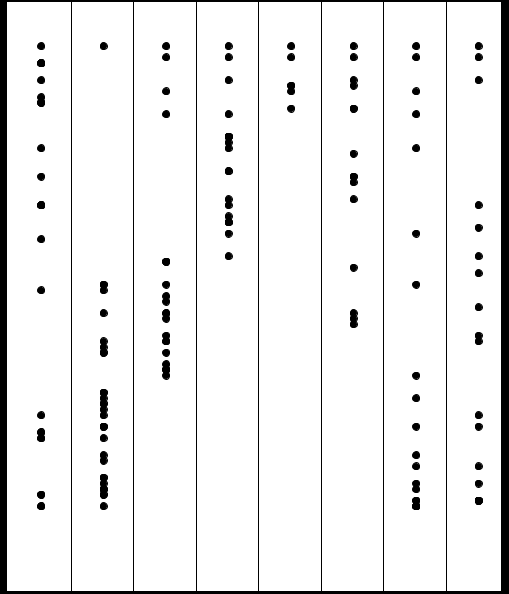
\includegraphics[scale=0.25]{Images/4By8MidTriOne.png} & 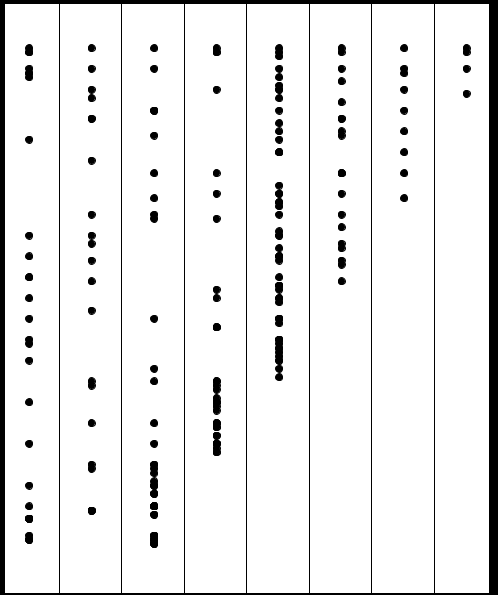
\includegraphics[scale=0.25]{Images/3By8LeftOne.png}
\end{tabular}
\end{center}
\caption{In the images, the cars are moving from top to bottom with the tollbooths at the top of the images. The left image represents our exotic new toll plaza design while the image of the right is a more standard toll plaza.}
\label{two_types}
\end{figure}

This simple design creates a powerful effect. By allowing the drivers to choose where they must go, and then holding them to that decision, we guide them towards more globally optimal choices. Since they must make important, lasting choices, socially harmful actions caused by aggressive over optimization are avoided. This improves the toll plaza on many fronts. It has better safety: fewer accidents happen. It has higher throughput: fewer cars go through the system. Travel times are faster: when drivers feel safer, they drive faster. And amazingly, it saves on cost. The creation of a space in the middle creates opportunity for rest stops and convenience stores. This will earn revenue, and it will improve the life of the drivers. 

We came to this conclusion using a model which is simple in idea: we created various different prototype designs, then used advanced artificial intelligence to simulate individual cars driving through the system. Each toll plaza has been tested for hundreds of thousands of hours by our advanced simulator, giving us confidence in our assumptions. Using this artificial intelligence, we have been able to simulate having autonomous, or self-driving vehicles, passing through the toll plaza as well. This ensures that our toll plaza designs are prepared for the future. 

We believe that by our innovations, the world will be made a better place. Never again will long traffic lines build up at toll spaces. Never again will it be slow. And never again will you not be able to stop for a break after a harrowing and horrible experience through a toll zone. These advances represent a quantum leap in toll plaza design, and we hope, for the good of humanity, that you adopt our design.

\

Thank you, 

The Traffic Engineers of the NJTA

\newpage



\bibliography{references.bib}
\bibliographystyle{plain}




\end{document}